\let\negmedspace\undefined
\let\negthickspace\undefined
\documentclass[journal]{IEEEtran}
\usepackage[a5paper, margin=10mm, onecolumn]{geometry}
%\usepackage{lmodern} % Ensure lmodern is loaded for pdflatex
\usepackage{tfrupee} % Include tfrupee package

\setlength{\headheight}{1cm} % Set the height of the header box
\setlength{\headsep}{0mm}     % Set the distance between the header box and the top of the text

\usepackage{gvv-book}
\usepackage{gvv}
\usepackage{cite}
\usepackage{amsmath,amssymb,amsfonts,amsthm}
\usepackage{algorithmic}
\usepackage{graphicx}
\usepackage{textcomp}
\usepackage{xcolor}
\usepackage{txfonts}
\usepackage{listings}
\usepackage{enumitem}
\usepackage{mathtools}
\usepackage{gensymb}
\usepackage[breaklinks=true]{hyperref}
\usepackage{tkz-euclide} 
\usepackage{listings}
% \usepackage{gvv}                                        
\def\inputGnumericTable{}                                 
\usepackage[latin1]{inputenc}                                
\usepackage{color}                                            
\usepackage{array}                                            
\usepackage{longtable}                                       
\usepackage{calc}                                             
\usepackage{multirow}                                         
\usepackage{hhline}                                           
\usepackage{ifthen}                                           
\usepackage{lscape}
\usepackage{circuitikz}
\usepackage{comment}
\tikzstyle{block} = [rectangle, draw, fill=blue!20, 
    text width=4em, text centered, rounded corners, minimum height=3em]
\tikzstyle{sum} = [draw, fill=blue!10, circle, minimum size=1cm, node distance=1.5cm]
\tikzstyle{input} = [coordinate]
\tikzstyle{output} = [coordinate]


\begin{document}

\bibliographystyle{IEEEtran}
\vspace{3cm}

\title{12.456}
\author{EE25BTECH11026-Harsha}
 \maketitle
% \newpage
% \bigskip
{\let\newpage\relax\maketitle}

\renewcommand{\thefigure}{\theenumi}
\renewcommand{\thetable}{\theenumi}
\setlength{\intextsep}{10pt} % Space between text and floats


\numberwithin{equation}{enumi}
\numberwithin{figure}{enumi}
\renewcommand{\thetable}{\theenumi}

\textbf{Question}:\\
If a rectangle is deformed into a parallelogram of equal area by simple shear deformation (with shear strain $\gamma$) parallel to the abscissa, the displacement matrix is \underline{\hspace{2cm}}.
\begin{enumerate}
\begin{multicols}{2}
    \item $\myvec{1&&\gamma\\0&&1}$
    \item $\myvec{1&&0\\\gamma&&1}$
    \item $\myvec{1&&0\\0&&1}$
    \item $\myvec{0&&\gamma\\1&&0}$
\end{multicols}
\end{enumerate}
\solution \\
Let us solve the given question theoretically and then verify the solution computationally.\\
\\
Due to the shear deformation, let $x',y'$ be the new coordinates. As the deformation is along the direction of abscissa,
\begin{align}
    \therefore y'=y \label{eq:1}
\end{align}
Let the displacement due to the shear deformation be $\Delta h$.
\begin{align}
    \gamma=\frac{\Delta h}{y}
\end{align}
\begin{align}
    \therefore \Delta h=\gamma y
\end{align}
\begin{align}
    \implies x'=x+\Delta h=x+\gamma y \label{eq:2}
\end{align}
From ~\eqref{eq:1} and ~\eqref{eq:2},
\begin{align}
    \therefore \myvec{x'\\y'}=\myvec{x+\gamma y \\ y}=\myvec{1&&\gamma\\0&&1}\myvec{x\\y}
\end{align}
\newpage
\vspace*{0.25cm}
From the figure, it is clearly verified that the theoretical solution matches with the computational solution.\\
\begin{figure}[H]
    \centering
    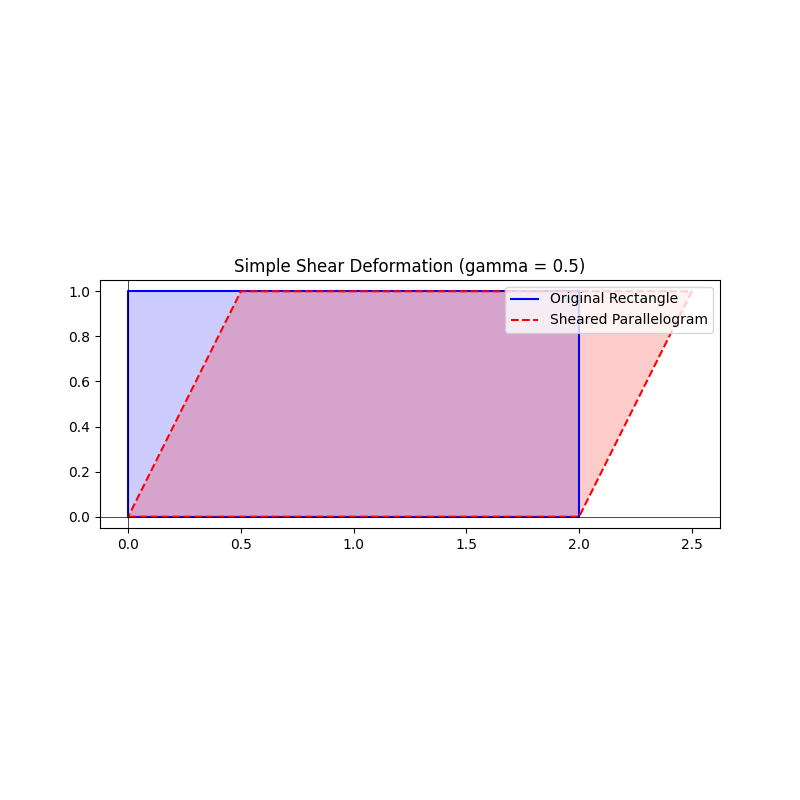
\includegraphics[width=0.8\columnwidth]{figs/Figure_1.png}
    \label{fig:1}
\end{figure}


\end{document}
